\documentclass[compress,t]{beamer}
%\usepackage[utf8]{inputenc}
\usetheme{Warsaw}
\usetheme{bcamath}

%\usepackage{amsfonts}
%\usepackage{amssymb}
%\usepackage{latexsym}
%\usepackage{textcomp}
\usefonttheme[onlymath]{serif}
\usepackage[justification=centering]{caption}

\title{\textit{Wave maker modelling\\ Numerical solver for Peregrine system}}
\author{Robin Goix}

\begin{document}
	\begin{frame}
		\titlepage
	\end{frame}
	\section{Motivations and goals}
		\begin{frame}
  			\begin{figure}
  				\movie[autoplay, loop]
				{\includegraphics[height=6cm]{Wavegarden2.jpeg}}{Wave.mp4}
				\caption{Wavegarden\\ \begin{scriptsize}Source: Youtube.(2014, Jan. 30) WAVE GARDEN avec SURF REPORT\end{scriptsize}}
				\end{figure}
		\end{frame}
  
		\begin{frame}
	 		\textbf{Wavegarden's Technology: an underwater object pulled in pool}
			\begin{figure}[H]
				\includegraphics[trim = 0 150 0 0, clip, height=2.1cm]{Wavegarden}
      			\caption{Wavegarden - Wake of the object\\ \begin{scriptsize}Source: \copyright 2014 Instant Sport S.L.\end{scriptsize}}
				\begin{minipage}[b]{0.46\linewidth}		
					\includegraphics[height=2cm]{Patent}\hfill
      			\caption{Underwater moving Object}	
				\end{minipage}			      	
      		\begin{minipage}[b]{0.46\linewidth}
      		\includegraphics[height=2cm]{Patent2}
      		\caption{The entire apparatus}
      		\end{minipage}
  	 		\end{figure}
		\end{frame}
  
		\begin{frame}
  			\vfill
			\begin{itemize}
				\item A recent but proven technology
				\item Made by surfers and engineers
				\item Build according to experience, intuition and real experimentation
			\end{itemize}
			\vfill
			\pause
			\textbf{Wavemaker project main goals}: 
			\begin{itemize}
				\item Model this phenomenon
				\item Optimize the shape of the moving object to obtain the best wave according to criteria to be determined (high, shape, ...) 
			\end{itemize}
			\vfill
		\end{frame}
  
  		\begin{frame}
			\tableofcontents
		\end{frame}
	\section{Saint-Venant equations as a first model}
  			\begin{frame}
				\begin{figure}
				\centering
 					\begin{minipage}[t]{0.3\linewidth}
 					\centering
 						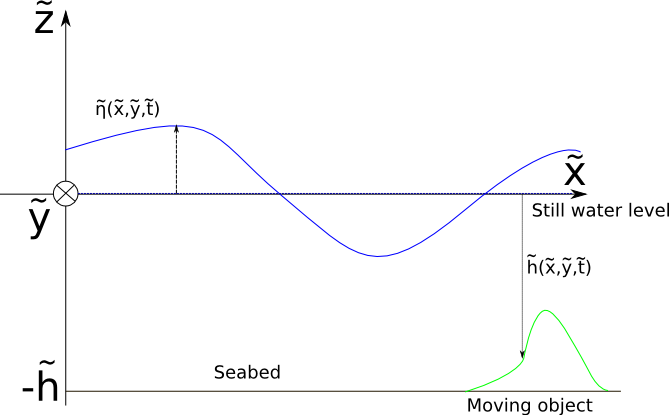
\includegraphics[height=2.7cm]{CartesianCoordinates}
						\caption{Reference}
 					\end{minipage} \hfill
 					\begin{minipage}[b]{0.6\linewidth}
 						\begin{itemize}
							\item Seabed profil: $\tilde h(\tilde x,\tilde y,\tilde t) = \tilde D(\tilde x,\tilde y) +\tilde  \zeta(\tilde x,\tilde y,\tilde t)$
							\item Free surface: $\tilde{\eta}(\tilde x,\tilde y,\tilde t)$
							\item Fluid velocity: $\hat{\mathbf{u}}(\tilde x,\tilde y,\tilde z,\tilde t)=(\tilde u,\tilde v,\tilde w)$
						\end{itemize}
 					\end{minipage}
				\end{figure}
				\pause
				Kinematic boundary conditions: 
				$\begin{array}{lr}
					\dfrac{\mathrm{d}}{\mathrm{d} \tilde t} \tilde  \eta(\tilde x,\tilde y,\tilde t) = \tilde w(\tilde x,\tilde y, \tilde \eta) & -\dfrac{\mathrm{d}}{\mathrm{d} \tilde t} \tilde h(\tilde x, \tilde y, \tilde t) = \tilde w(\tilde x,\tilde y,\tilde h)
				\end{array}$
			\end{frame}
  			\begin{frame}
  				\vfill
				\begin{itemize}
					\item The fluid is incompressible and inviscid;
					\item The typical water depth $h_0$ is small compare to the horizontal scale $\lambda_0$, i.e. $\sigma = \frac{h_0}{\lambda_0} \ll 1 $;
					\item The horizontal velocity $\hat{\mathbf{u}}_h = (\tilde u, \tilde v)$ is \textbf{independent} of $\tilde z$.
				\end{itemize}
				\vfill
				\pause
 				Euler equations are: 
				\begin{align*}
						\displaystyle \mathbf{\hat{u}}_{\tilde{t}} + (\mathbf{\hat{u}} \cdot \tilde{\nabla}) \mathbf{\hat{u}} + \frac{1}{\rho} \tilde{\nabla}\tilde{P} &=  -\mathbf{g}\\
						\tilde{\nabla} \cdot \mathbf{\hat{u}} & = 0 \\
				\end{align*}	
				\vfill	
			\end{frame}
			
  			\begin{frame}
  				Scaling: 
  				\begin{equation*}
					x = \frac{\tilde{x}}{\lambda_0},\; 
					y = \frac{\tilde{y}}{\lambda_0}, \;
					z = \frac{\tilde{z}}{h_0}, \; 
					t = \frac{c_0}{\lambda_0}\tilde{t},\;
					P = \dfrac{\tilde{P}}{\rho c_0^2},\;
					h = \dfrac{\tilde{h}}{h_0}	
				\end{equation*}
				\begin{equation*}
					u = \frac{h_0}{a_0 c_0} \tilde{u},\;
					v = \dfrac{h_0}{a_0 c_0} \tilde{v},\;
					w = \dfrac{\lambda_0}{a_0 c_0} \tilde{w},\; 
					\eta = \dfrac{\tilde{\eta}}{a_0},\;
					D = \dfrac{\tilde{D}}{h_0}, \;
					\zeta = \dfrac{\tilde{\zeta}}{a_0}			
				\end{equation*}
				with $c_0 = \sqrt{h_0 g}$, and $\epsilon = a_0/h_0$.\\ 
				\vfill		
				\pause
				We finally obtain: 
				\begin{align*}
					\mathbf{u}_t + \nabla\eta + \epsilon (\mathbf{u} \cdot \nabla) \mathbf{u} &= 0 \\
					\eta_t + \zeta_t + \nabla \cdot [(h+\epsilon \eta) \mathbf{u}] &= 0
				\end{align*}
				\vfill
			\end{frame}
			
  			\begin{frame}
				\begin{figure}
					\begin{minipage}[b]{0.4\linewidth}
					  	\movie[autoplay]
						{\includegraphics[height=2.5cm]{SWECircle.png}}{SWECircle.ogv}
					\end{minipage}
					\hfill
					\begin{minipage}[b]{0.4\linewidth}
					  	\movie[autoplay]
						{\includegraphics[height=2.5cm]{SWEMovingBottom}}{SWEMovingBottom.ogv}
					\end{minipage}\\
					\begin{minipage}{0.9\linewidth}
						\caption{Numerical solver of shallow water equations}
					\end{minipage}
  				\end{figure}
  				\vfill
  				\pause
  				The main assumption (the horizontal velocity does not depend on $z$) is constraining. We may want to find a more accurate model. 
  				\vfill
  			\end{frame}
	\section{A second model: Peregrine system}
  			\begin{frame}
 				\begin{figure}
 					\begin{minipage}[t]{0.3\linewidth}
 						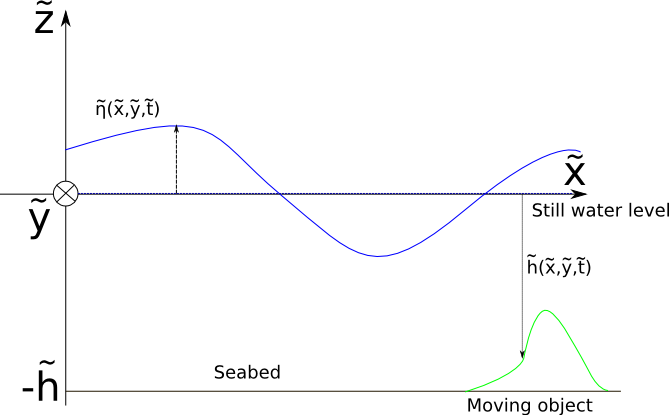
\includegraphics[height=2.7cm]{CartesianCoordinates}
						\caption{Reference}
 					\end{minipage} \hfill
 					\begin{minipage}[b]{0.6\linewidth}
 						\begin{itemize}
							\item Seabed profil: $\tilde h(\tilde x,\tilde y,\tilde t) = \tilde D(\tilde x,\tilde y) +\tilde  \zeta(\tilde x,\tilde y,\tilde t)$
							\item Free surface: $\tilde{\eta}(\tilde x,\tilde y,\tilde t)$
							\item Fluid velocity: $\hat{\mathbf{u}}(\tilde x,\tilde y,\tilde z,\tilde t)=(\tilde u,\tilde v,\tilde w)$
						\end{itemize}
 					\end{minipage}
				\end{figure}
				\pause
				Scaling: 
  				\begin{equation*}
					x = \frac{\tilde{x}}{\lambda_0},\; 
					y = \frac{\tilde{y}}{\lambda_0}, \;
					z = \frac{\tilde{z}}{h_0}, \; 
					t = \frac{c_0}{\lambda_0}\tilde{t},\;
					P = \dfrac{\tilde{P}}{\rho c_0^2},\;
					h = \dfrac{\tilde{h}}{h_0}	
				\end{equation*}
				\begin{equation*}
					u = \frac{h_0}{a_0 c_0} \tilde{u},\;
					v = \dfrac{h_0}{a_0 c_0} \tilde{v},\;
					w = \dfrac{\lambda_0}{a_0 c_0} \tilde{w},\; 
					\eta = \dfrac{\tilde{\eta}}{a_0},\;
					D = \dfrac{\tilde{D}}{h_0}, \;
					\zeta = \dfrac{\tilde{\zeta}}{a_0}			
				\end{equation*}
			\end{frame}
 	
			\begin{frame}
 				Dimensionless form of the Euler equations and irrotationality: 
				\begin{align*}
					\epsilon \mathbf{u}_t + \epsilon^2((\mathbf{u} \cdot \nabla) \mathbf{u} + w \mathbf{u}_z) + \nabla P & = 0\\
					\epsilon \sigma^2 w_t + \epsilon^2 \sigma^2 ((\mathbf{u} \cdot \nabla w) + w w_z) + P_z & = -1 \\
					\nabla \cdot \mathbf{u} + w_z & =  0 \\
					u_y-v_x & = 0 \\
					\mathbf{u}_z - \sigma^2 \nabla w & = 0
				\end{align*}
				Dimensionless form of the boundary conditions: 
				\begin{align*}
					\eta_t + \epsilon (\mathbf{u} \cdot \nabla \eta ) & = w & \mathrm{on} \: z = \epsilon \eta\\
					- \zeta_t - \mathbf{u} \cdot \nabla h & = w & \mathrm{on} \:  z = -h
				\end{align*}
 			\end{frame}
 	
 			\begin{frame}
 				Integration: $\displaystyle \nabla \cdot \mathbf{u} + w_z =  0 \Rightarrow w = -\mathbf{u} \cdot \nabla h - \int^z_{-h} \nabla \cdot \mathbf{u} - \zeta_t $
				Integration: $	\mathbf{u}_z - \sigma^2 \nabla w  = 0 \Rightarrow \mathbf{u} = \mathbf{u}_b + O(\sigma^2)$
				
				\pause
				Using:		
				\begin{equation*}
					\left\lbrace
						\begin{aligned}
							w = -\mathbf{u} \cdot \nabla h - \int^z_{-h} \nabla \cdot \mathbf{u} - \zeta_t \\
							\mathbf{u}_z - \sigma^2 \nabla w  = 0 \\
							\mathbf{u} = \mathbf{u}_b + O(\sigma^2)
						\end{aligned}
					\right.
				\end{equation*}
				and integrating, we obtain:
				\begin{align*}
					\mathbf{u} = & \mathbf{u}_b 
					\only<2>{- \sigma^2(z+h)\nabla (\nabla \cdot (h \mathbf{u}_b)) - \sigma^2 \frac{z^2-h^2}{2}\nabla ( \nabla \cdot \mathbf{u}_b)} 
					\only<3>{\textcolor{blue}{- \sigma^2(z+h)\nabla (\nabla \cdot (h \mathbf{u}_b)) - \sigma^2 \frac{z^2-h^2}{2}\nabla ( \nabla \cdot \mathbf{u}_b)}} \\
					& \quad 
					\only<2>{- \sigma^2(z+h)\nabla \zeta_t + O(\sigma^4)}
					\only<3>{\textcolor{blue}{- \sigma^2(z+h)\nabla \zeta_t + O(\sigma^4)}}
				\end{align*}
 			\end{frame}
 			
 			\begin{frame}
  				We finally obtain the following system, which is similar to the Boussinesq System derived by Peregrine:
  				\begin{center}
					$\left\lbrace
						\begin{array}{rll}
							\displaystyle \mathbf{u}_t + \nabla \eta + \epsilon (\mathbf{u} \cdot \nabla)\mathbf{u} \only<1>{- \sigma^2\frac{h}{2}\nabla (\nabla \cdot (h \mathbf{u}_t))}
							\only<2>{\textcolor{blue}{- \sigma^2\frac{h}{2}\nabla (\nabla \cdot (h \mathbf{u}_t))}}
							& & \\
							\only<1>{+ \displaystyle \sigma^2 \frac{h^2}{6}\nabla (\nabla \cdot \mathbf{u}_t) - \sigma^2\frac{h}{2}\nabla \zeta_{tt}}
							\only<2>{\textcolor{blue}{+ \displaystyle \sigma^2 \frac{h^2}{6}\nabla (\nabla \cdot \mathbf{u}_t) - \sigma^2\frac{h}{2}\nabla \zeta_{tt}}} & = & \displaystyle O(\epsilon \sigma^2, \sigma^4) \\ [10pt]
							\displaystyle \eta_t+\zeta_t + \nabla \cdot [(h+\epsilon\eta)\mathbf{u}] & = & 0
						\end{array}
					\right.$ \\[15pt]
					\only<2>{\textbf{Shallow Water Equations}}	
				\end{center}
				\vfill
				\pause
				$\rightarrow$ A Taylor series expansion one-order more accurate
				\vfill
			\end{frame}
			
	\section{Simulations and results}
			\begin{frame}
				We are looking for a weak formulation for this system: 
				\begin{equation*}
					\begin{array}{rlr}
						\mathbf{u}_t + \nabla \eta + \epsilon (\mathbf{u} \cdot \nabla)\mathbf{u} - \sigma^2\dfrac{h}{2}\nabla (\nabla \cdot (h \mathbf{u}_t)) & & \\
						+ \sigma^2 \dfrac{h^2}{6}\nabla (\nabla \cdot \mathbf{u}_t) - \sigma^2\dfrac{h}{2}\nabla \zeta_{tt}  & = O(\epsilon \sigma^2, \sigma^4) & \only<3->{\int_{\Omega}[\; \bullet \; \cdot \mathbf{v}]}\\
					\eta_t+\zeta_t + \nabla \cdot [(h + \epsilon\eta )\mathbf{u} ] & = 0 & \only<3->{\int_{\Omega}[\; \bullet \; \xi]}
					\end{array}	
				\end{equation*}
				\pause
				Let $(\mathbf{v},\xi) \in \mathbb{H}^1_0(\Omega)^2 \times \mathbb{H}^1(\Omega)$.
				\pause
				\pause 
				\begin{small}
					\begin{equation*}
						\begin{split}
							\int_{\Omega} \! \mathbf{u}_t \cdot \mathbf{v} \: \mathrm{dx} + \int_{\Omega} \! \nabla \eta \cdot \mathbf{v} \: \mathrm{dx} + \epsilon \! \int_{\Omega} \! (\mathbf{u} \cdot \nabla ) \mathbf{u} \cdot \mathbf{v} \: \mathrm{dx} - \sigma^2 \! \int_{\Omega} \! \frac{h}{2} \nabla (\nabla \cdot (h \mathbf{u}_t)) \cdot \mathbf{v} \: \mathrm{dx} \\
							+ \sigma^2 \! \int_{\Omega} \! \frac{h^2}{6} \nabla (\nabla \cdot \mathbf{u}_t) \cdot \mathbf{v} \: \mathrm{dx} - \sigma^2 \! \int_{\Omega} \! \frac{h}{2} \nabla \zeta_{tt} \cdot \mathbf{v} \: \mathrm{dx} = 0\\
							\int_{\Omega}\! \eta_t \; \xi \: \mathrm{dx} +\int_{\Omega}\! \zeta_t \; \xi \: \mathrm{dx} +\int_{\Omega}\! \nabla \cdot [(h+\epsilon\eta) \mathbf{u}] \; \xi \: \mathrm{dx} = 0
						\end{split}
					\end{equation*}
				\end{small}		  
			\end{frame}
			\begin{frame}
				Using divergence theorem and the fact that $\mathbf{v}$ and $\mathbf{u}$ vanish on the boundaries, we get: 
				\begin{scriptsize}
					\begin{equation*}
						\begin{split}
							0 &= \int_{\Omega} \! \mathbf{u}_t \cdot \mathbf{v} \: \mathrm{dx} - \int_{\Omega} \! \eta \; (\nabla \cdot \mathbf{v}) \: \mathrm{dx} + \epsilon \! \int_{\Omega} \! (\mathbf{u} \cdot \nabla ) \mathbf{u} \cdot \mathbf{v} \: \mathrm{dx} + \frac{\sigma^2}{2} \! \int_{\Omega} \!  (\nabla \cdot (h \mathbf{u}_t)) \; (\nabla \cdot (h \mathbf{v}) )\: \mathrm{dx} \\
							&\quad - \frac{\sigma^2}{6} \! \int_{\Omega} \! (\nabla \cdot \mathbf{u}_t) \; (\nabla  \cdot (h^2  \mathbf{v})) \: \mathrm{dx} + \frac{\sigma^2}{2} \! \int_{\Omega} \!  \zeta_{tt}  \; (\nabla \cdot( h \mathbf{v})) \: \mathrm{dx}\\
							0 &= \int_{\Omega}\! \eta_t \; \xi \: \mathrm{dx} +\int_{\Omega}\! \zeta_t \; \xi \: \mathrm{dx} -\int_{\Omega}\! \nabla \xi \; \cdot [(h+\epsilon\eta) \mathbf{u}]  \: \mathrm{dx}
						\end{split} 
					\end{equation*}
				\end{scriptsize}
				Noticing that $\frac{\partial h}{\partial t} = \epsilon \frac{\partial \zeta}{\partial t}$, we finally obtain: 
				\begin{scriptsize}
					\begin{equation*}
						\begin{split}
							0 &= \int_{\Omega} \! \mathbf{u}_t \cdot \mathbf{v} \: \mathrm{dx} - \int_{\Omega} \! \eta \; (\nabla \cdot \mathbf{v}) \: \mathrm{dx} + \epsilon \! \int_{\Omega} \! (\mathbf{u} \cdot \nabla ) \mathbf{u} \cdot \mathbf{v} \: \mathrm{dx} + \frac{\sigma^2}{2} \! \int_{\Omega} \!  (\nabla \cdot (h 
\mathbf{u}_t)) \; (\nabla \cdot (h \mathbf{v}) )\: \mathrm{dx} \\ 
							&\quad - \frac{\sigma^2}{6} \! \int_{\Omega} \! (\nabla \cdot \mathbf{u}_t) \; (\nabla  \cdot (h^2  \mathbf{v})) \: \mathrm{dx} + \frac{\sigma^2}{2 \epsilon} \! \int_{\Omega} \!  h_{tt}  \; (\nabla \cdot( h \mathbf{v})) \: \mathrm{dx}\\
							0 &= \int_{\Omega}\! \eta_t \; \xi \: \mathrm{dx} +\frac{1}{\epsilon}\int_{\Omega}\! h_t \; \xi \: \mathrm{dx} -\int_{\Omega}\! \nabla \xi \; \cdot [(h+\epsilon\eta) \mathbf{u}]  \: \mathrm{dx}
						\end{split}
					\end{equation*}
				\end{scriptsize}
			\end{frame}
			
			\begin{frame}
			\vfill
			With a time discretization, For each time-step, knowing $\mathbf{u}^{n-1}$ and $\eta^{n-1}$, our problem is therefore:\\
			\vfill
			Find $(u,\eta) \in \mathbb{H}^1_0(\Omega)^2 \times \mathbb{H}^1(\Omega), \forall (v,\xi) \in \mathbb{H}^1_0(\Omega)^2 \times \mathbb{H}^1(\Omega)$:  
				\begin{scriptsize}
					\begin{equation*}
						\begin{split}
							0 &= \int_{\Omega} \! \frac{\mathbf{u} - \mathbf{u}^{n-1}}{\mathrm{dt}} \cdot \mathbf{v} \: \mathrm{dx} 	- \int_{\Omega} \! \eta \; (\nabla \cdot \mathbf{v}) \: \mathrm{dx} + 	\epsilon \! \int_{\Omega} \! (\mathbf{u} \cdot \nabla ) \mathbf{u} \cdot \mathbf{v} \: \mathrm{dx} + \frac{\sigma^2}{2 \epsilon} \! \int_{\Omega} \!  h_{tt}  \; (\nabla \cdot( h \mathbf{v})) \: \mathrm{dx} \\ 
					&\quad + \frac{\sigma^2}{2} \! \int_{\Omega} \!  (\nabla \cdot (h \frac{\mathbf{u} - \mathbf{u}^{n-1}}{\mathrm{dt}})) \; (\nabla \cdot (h \mathbf{v}) )\: \mathrm{dx} - \frac{\sigma^2}{6} \! \int_{\Omega} \! (\nabla 	\cdot \frac{\mathbf{u} - \mathbf{u}^{n-1}}{\mathrm{dt}}) \; (\nabla  \cdot (h^2  \mathbf{v})) \: \mathrm{dx} \\
					\displaystyle 0 &= \int_{\Omega}\! \frac{\eta - \eta^{n-1}}{\mathrm{dt}} \; \xi \: \mathrm{dx} +\frac{1}{\epsilon}\int_{\Omega}\! h_t \; \xi \: \mathrm{dx} - \int_{\Omega}\! \nabla \xi \; \cdot [(h+\epsilon\eta) \mathbf{u}]  \: 	\mathrm{dx}
				\end{split}
			\end{equation*}
				\end{scriptsize}
				\vfill
			\end{frame}
			
			\begin{frame}
			\textbf{Computational framework}
				\begin{figure}
				\centering
					\begin{minipage}[b]{0.49\linewidth}
						\centering
						\includegraphics[height=1.5cm]{FenicsProject}		
					\end{minipage}
					\hfill
					\begin{minipage}[b]{0.49\linewidth}
						\centering
						\includegraphics[height=1.5cm]{Dolfin}
					\end{minipage}\\[-7pt]
					\begin{minipage}[t]{0.49\linewidth}
						\centering
						\caption{FEniCS}
					\end{minipage}
					\hfill
					\begin{minipage}[t]{0.49\linewidth}
						\centering
						\caption{Dolfin}
					\end{minipage}
				\end{figure}
				\begin{figure}	
				\centering
					\begin{minipage}[b]{0.6\linewidth}
					\centering
						\includegraphics[height=1.3cm]{Pool}
						\caption{Pool's dimensions}
					\end{minipage}\hfill
					\begin{minipage}[b]{0.3\linewidth}
					\centering
						\includegraphics[height=1.5cm]{PoolMesh}
						\caption{Refined mesh}
					\end{minipage}
				\end{figure}								
				\begin{tabular}{l|r}
					Finite-Elements spaces & P2 $\times$ P1 \\				
				\end{tabular}				
			\end{frame}
			
			\begin{frame}
				\begin{figure}
					\begin{minipage}{0.3\linewidth}
						\begin{tabular}{l|r}
							\hline
							time step & 0.03 s \\
							Pool & 30 x 44 m$^2$ \\
							depth & 1 m \\
							Object $a_0$ & 0.4 m\\
							Vmax & $\sqrt{g(h_0 + a_0)}$ \\
							\hline
						\end{tabular}
					\end{minipage}
					\hfill
					\begin{minipage}{0.5\linewidth}
						\movie[autoplay, loop]
						{\includegraphics[height=2.9cm]{RealSizeV-Shape1}}{RealSizeSimulationV-Shape1.ogv}
					\end{minipage}
				\end{figure}
				\begin{figure}
					\begin{minipage}{0.3\linewidth}
						\includegraphics[height=3cm]{BottomVShape1-2}
						\caption{Object's Shape}
					\end{minipage}
					\hfill
					\begin{minipage}{0.5\linewidth}
						\movie[autoplay, loop]
						{\includegraphics[height=3cm]{LongPoolSimulation}}{LongPoolSimulationV-Shape.ogv}
					\end{minipage}
				\end{figure}
			\end{frame}
						
	\section{Several problems we are facing}				
		\begin{frame}
			\textbf{Instability \& breaking wave problem}\\
			\begin{center}
  				\movie[autoplay, loop]
				{\includegraphics[height=4cm]{Peregrine3}}	{BreakingWaveIssue.ogv}
				\end{center}
		\end{frame}
		
		\begin{frame}
			\textbf{Limits of the Peregrine model}\\
			\begin{figure}
				\begin{minipage}[b]{0.4\linewidth}
					\includegraphics[height=2cm]{Peregrine3}
					\caption{Start of the object's motion}
				\end{minipage}
				\hfill
				\begin{minipage}[b]{0.45\linewidth}
					\includegraphics[height=2cm]{PeregrineSteepObject}
					\caption{Object's wake}
				\end{minipage}
			\end{figure}

			\pause
			\begin{center}
					$\left\lbrace
						\begin{array}{rll}
							\displaystyle \mathbf{u}_t + \nabla \eta + \epsilon (\mathbf{u} \cdot \nabla)\mathbf{u} - \sigma^2\frac{h}{2}\nabla (\nabla \cdot (h \mathbf{u}_t))
							& & \\
							+ \displaystyle \sigma^2 \frac{h^2}{6}\nabla (\nabla \cdot \mathbf{u}_t) - \sigma^2\frac{h}{2}\nabla \zeta_{tt} & = & \displaystyle O(\only<2>{\epsilon} \only<3>{\textcolor{red}{\mathbf{\epsilon}}} \sigma^2, \sigma^4) \\
							\displaystyle \eta_t+\zeta_t + \nabla \cdot [(h+\epsilon\eta)\mathbf{u}] & = & 0
						\end{array}
					\right.$ \\
				\end{center}
		\end{frame}
		
		\begin{frame}
			\centering 
			\vfill
				Next step: \textbf{optimisation} problem\\
				\vfill
			\begin{huge}
				Thank you for your attention!
			\end{huge}
			\vfill
		\end{frame}
\end{document}